\begin{figure}[htbp]\centering
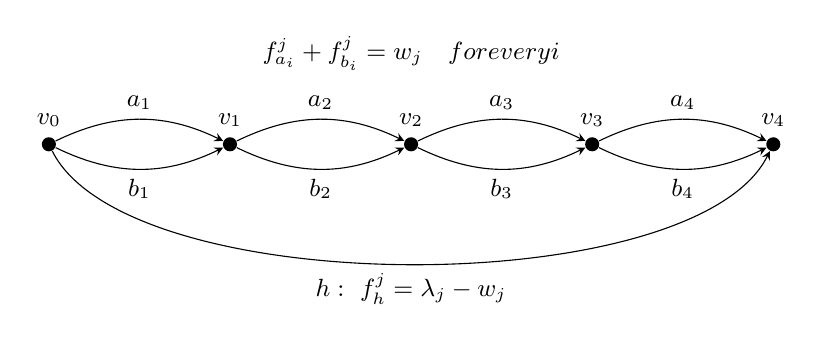
\begin{tikzpicture}[>=stealth,vertex/.style={circle,fill=black,inner sep=1.8pt},
                   every node/.style={font=\small}]
\foreach \i in {0,...,4}{
  \node[vertex,label=above:{$v_\i$}] (v\i) at (2.3*\i,0) {};
}
\foreach \i [evaluate=\i as \prev using int(\i-1)] in {1,...,4}{
  \draw[->] (v\prev) to[bend left=26] node[above] {$a_\i$} (v\i);
  \draw[->] (v\prev) to[bend right=26] node[below] {$b_\i$} (v\i);
}
\draw[->] (v0) .. controls (1,-2.0) and (8.2,-2.0) ..
  node[below] {$h:\ f_h^j=\lambda_j-w_j$} (v4);
\node at (4.6,1.15) {$f_{a_i}^j+f_{b_i}^j=w_j\quad\text{for every }i$};
\end{tikzpicture}
\caption{The flat chain $G_4$. Each serial pair carries the same statewise
branch flow $w_j$; the bypass carries the remainder. All capacities and the
source--sink flow value are one. Independent scalar totals at the four pairs
do not retain the common vector of state flows. The general $G_L$ extends
the same pattern to $L$ pairs.}\label{fig:flat-chain}
\end{figure}
